\documentclass[../CSC_52081_EP.tex]{subfiles}

\begin{document}
\section{Results and Discussion}

\subsection{CEM}

Figure \ref{fig:train_plot} shows the evolution of the training rewards over iterations for the CEM algorithm. As expected from the minimization strategy applied in our implementation, the reward value starts at a high level and decreases steadily, eventually stabilizing between 5 and 10. This behavior indicates that the algorithm is correctly minimizing the cost, since our objective function returns the negative reward.

\begin{figure}[H]
    \centering
    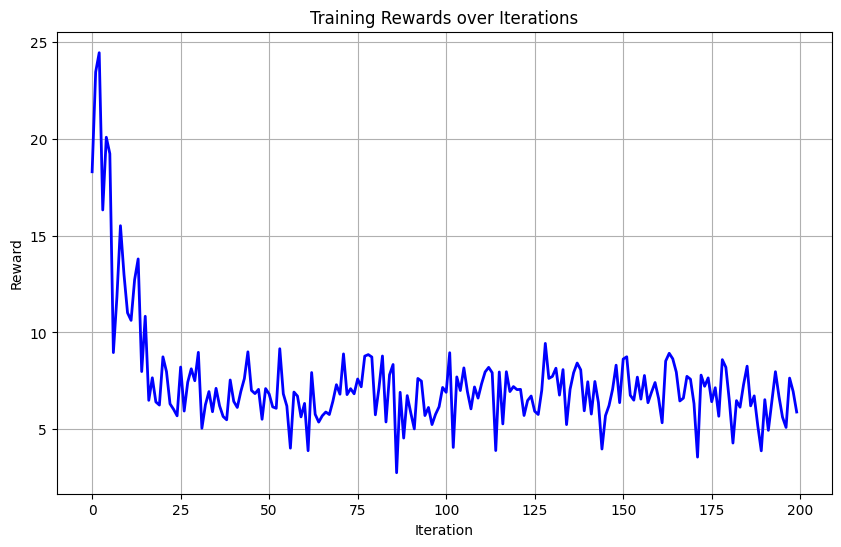
\includegraphics[width=0.3\textwidth]{figures/CEM_train.png}
    \caption{Training plot showing the evolution of the reward over iterations.}
    \label{fig:train_plot}
\end{figure}

However, the desired outcome was to achieve a much lower (more negative) reward value as training progressed, which would have translated into better performance by the agent when navigating the track. Unfortunately, the final model did not produce the expected results in the environment, as demonstrated by the video reproduction of the car on the track.

This may be the result of some problems with the model. One possibility is that the reward structure, when negated for minimization, may be inadvertently favoring a strategy that minimizes penalization rather than encouraging forward progress. Additionally, the parameters of the CNN or the action scaling (especially for the steering, gas, and brake outputs) might not be appropriately tuned, causing the policy to output nearly constant or ineffective actions. Overall, these factors combined may result in the agent exploiting a trivial strategy that minimizes the cost, rather than discovering a policy that drives effectively along the track. But, despite this problem, the training plot confirms that the minimization mechanism is operating as designed.

\end{document}
